\chapter{Applications to Elliptic equations}

	
Let $X_t$ be the solution to \eqref{eq:sde} with $X_0=x$. We will write $\left(\mathbb{P}_x, X_t\right)$ for the strong Markov process corresponding to $\sigma$ and $b$ (This can be ensured by assuming $\sigma, b\in C^1_b$, or $a\in \mS_\delta$, $a$ is continuous and $b$ is bounded). 

Put \(L=a_{ij}\partial_{ij}+b_i\partial_i\). We always assume \(a\) and \(b\) are bounded. 
	
\section{Poisson equations}
Consider the following Poisson equation: 
\begin{equation}
    \lambda u - L u=f, \quad \lambda>0, f\in C_b. 
\end{equation}
The relationship between these two subjects can be easily established by It\^o's formula: 
\begin{theorem}\label{thm:FK1}
    Suppose $u$ is a $C^2_b$ function satisfying the above Poisson equation. Then
    \[
        u(x)=\mE_x \int_0^{\infty} e^{-\lambda t} f\left(X_t\right) \d t
    \]
\end{theorem}
\begin{proof}
    Applying It\^o's formula, we have $\d u(X_t)=\d M_t + Lu(X_t) \d t$, where \(M\) is a \(L^2\)-martingale. So 
    \[
        \begin{aligned}
            e^{-\lambda t} u\left(X_t\right)-u\left(x\right)=&\int_0^t e^{-\lambda s} \d M_s+\int_0^t e^{-\lambda s} L u\left(X_s\right) \d s \\
            &-\lambda \int_0^t e^{-\lambda s} u\left(X_s\right) \d s.
	\end{aligned}
    \]
Taking expectation, we get what we claimed. 
\end{proof}
	
Let us now let $D$ be a nice bounded domain, e.g., a ball. Poisson's equation in $D$ requires one to find a function $u$ such that 
	\begin{equation*}
		\begin{cases}
			\lambda u- Lu=f ~&\mbox{in}~ D\\
			u=0 ~&\mbox{on}~ \p D, 
		\end{cases}
	\end{equation*}
	where $\lambda\geq 0$. Here we can allow $\lambda$ to be equal to $0$. Recall that if $L=\Delta$ ($X_t$ is a Brownian motion), then the time to exit $D$, namely, $\tau_D := \inf\{t>0: X_t \notin D\}$, is finite almost surely. 
	
	\begin{theorem}\label{thm:PR-Dir}
		Suppose $u$ is a solution to Poisson's equation in a bounded domain $D$ that is $C^2$ in $D$ and continuous on $\bar{D}$. Assume also that 
		\begin{equation*}
			\mP_x(\tau_D<\infty)=1, \quad x\in D
		\end{equation*}
		where $\tau_D=\inf\{t>0: x\notin D\}$. Then
		\[
		    u(x)=\mathbb{E}_x \int_0^{\tau_D} e^{-\lambda s} f\left(X_s\right) \d s.		
		\]
	\end{theorem}
	\begin{exercise}
		Prove Theorem \ref{thm:PR-Dir}. 
	\end{exercise}
	
\section{Dirichlet Problems and Harmonic functions}
Let $D$ be a ball (or other nice bounded domain) and let us consider the solution to the Dirichlet problem: given $g$ a continuous function on $\p D$, find $u\in C(\bar D)$ such that $u$ is $C^2$ in $D$ and 
\begin{equation}\label{eq:DP}
    \begin{cases}
	Lu=0~\mbox{in}~ D\\
	u=g ~\mbox{on}~\p D. 
    \end{cases}
\end{equation}
If $Lu=0$ in $D$, we say $u$ is $L$-harmonic in $D$.

\begin{theorem}\label{thm:PR-DP}
    Assume that \(\mP_x(\tau_D<\infty)=1\) for each \(x\in D\). Suppose that \(u\in C^2(D)\cap C(\bar{D})\) satisfies \eqref{eq:DP}, then 
    $$
    u(x)=\mathbb{E}_x g\left(X_{\tau_D}\right). 
    $$
\end{theorem}
\begin{proof}
    Let $\tau_n=\inf \left\{t: \operatorname{dist}\left(X_t, \partial D\right)<1 / n\right\}$. By Itô's formula,
		$$
		u\left(X_{t \wedge \tau_n}\right)=u\left(X_0\right)+M_{t\wedge \tau_n}+\int_0^{t \wedge \tau_n} L u\left(X_s\right) d s .
		$$
		Since $L u=0$ inside $D$, taking expectations shows
		$$
		u(x)=\mathbb{E}_x u\left(X_{t \wedge \tau_n}\right) .
		$$
		We let $t \rightarrow \infty$ and then $n \rightarrow \infty$. By dominated convergence, we obtain $u(x)=\mathbb{E}_x u\left(X_{\tau_D}\right)$. This is what we want since $u=g$ on $\partial D$.
\end{proof}
	\begin{exercise}
		Theorem \ref{thm:PR-DP} implies the weak maximum principle: $\max_{D} u\leq \max_{\p D} u$. 
	\end{exercise}
	
	\begin{exercise}
		Theorem \ref{thm:support} implies the strong maximum principle: if $u$ is not a constant function, then for each  $x\in D$, $u(x)<\max_{\p D} u$
	\end{exercise}
	
	\begin{theorem}
		Assume that \((\mP_x, X_t)\) is a strong Markov process and that $\mP_x\l( \tau_D<\infty\r)=1$, \(x\in D\). Suppose that \(a,b\in C(D)\), $g\in C(\partial D)$, and $u(x):=\mE_x g(X_{\tau_D})\in C^2(D)$. Then $L u=0$ in $D$.
	\end{theorem}
\begin{proof}
    Let $B_r(x)\subseteq D$. By the strong Markov property, we have 
        \begin{align*}
          u(x)=&\mE_x g(X_{\tau_D})= \mE_x g(X_{\tau_{D}}\circ \theta_{\tau_{B_r(x)}})=\mE_x \l\{ \mE_x \l[ g(X_{\tau_{D}}\circ \theta_{\tau_{B_r(x)}})\Big|\cF_{\tau_{B_r(x)}}\r] \r\}\\
          =&\mE_x \l[ \mE_{X_{\tau_{B_r(x)}}} g(X_{\tau_D})\r]= \mE_x u(X_{\tau_{B_r(x)}}). 
        \end{align*}
     Noting that $u\in C^2(D)$, by It\^o's formula, 
     \[
         u(X_{t\wedge \tau_{B_r(x)}})-u(x) = \int_0^{t\wedge \tau_{B_r(x)}} L u (X_s) \d s+ M_{t\wedge \tau_{B_r(x)}}, 
     \]
     where $M$ is a martingale. Taking expectations and letting $t\to\infty$, 
     \[
        0= \frac{1}{\mE_x\tau_{B_r(x)}}\mE_x \int_0^{\tau_{B_r(x)}} L u(X_s) \d s.  
     \]
     By the continuity of $Lu$ and letting $r\to0$, we get $Lu(x)=0$. 
\end{proof}


    One can also consider the following Schrödinger type operator: 
    \[
      L_q u= Lu+cu. 
    \]
   Equation involving the above operator are considerably simpler than the quantum mechanics Schrödinger equation because here all terms are real-valued. 

   \begin{theorem}\label{thm:FK2}
       Let $D$ be a nice bounded domain, and $q\in C(\bar D)$ and $g\in C(\p D)$. Let $u\in C^2(D)\cap C(\bar D)$ that agrees with $g$ on $\p D$ and satisfies $L_q u=0$ in $D$. If 
       \[
          \mE_x \exp\l(\int_0^{\tau_D}q^+(X_s) \d s\r)<\infty, 
       \]
       then 
       \[
         u(x)=\mE_x \l[ g(X_{\tau_D})\exp\l(\int_0^{\tau_D}q(X_s) \d s\r)\r].
       \]
   \end{theorem}
   
\begin{exercise}
    Prove Theorem \ref{thm:FK2}. 
\end{exercise}
\begin{exercise}
    Using \eqref{eq:Kry1} to show: there exists $\varepsilon>0$ such that if $B \subseteq Q_1, x \in Q_{1/2}$, and $|Q_1-B|<\varepsilon$, then
    $$
    \mathbb{E}_x \int_0^{\tau_{Q_1}} 1_B\left(X_s\right) d s \geq c>0, 
    $$
    where $c$ is a constant only depends on $d,\delta$ and $\varepsilon$. 
\end{exercise}
	
\section{Once again on the hitting probability}
	Recall that 
	\[
	x_t=\int_0^t \sigma_s \d W_s, \quad a=\frac{1}{2}\sigma \sigma^t \in \mS^d_\delta. 
	\]
	
	In this section, we want to prove following important hitting probability estimate, which is a refined version of Proposition \ref{prop:hit}. This was first found by Krylov-Safonov \cite{krylov1979estimate}. 
	
	Recall that 
	\[
	    \sigma_{\Gamma}(x)= \inf\l\{t>0: x+x_t\in \Gamma\r\} ~\mbox{ and }~ \tau_Q= \inf\l\{t>0: x+x_t\notin Q\r\}. 
	\]
	\begin{theorem}\label{thm:hit}
		There is a increasing function $p: (0,1)\to (0,1)$, which only depends on $d$ and $\delta$, such that for any $\Gamma \subset Q_1$ and $x\in Q_{1/2}$,  
		\begin{equation}
			\bP (\sigma_\Gamma(x)<\tau_{Q_1}(x)) \geq p(|\Gamma|). 
		\end{equation}
	\end{theorem}
	
	Before prove Theorem \ref{thm:hit}, we need some preparation.  
	
	One tool is a corollary of the Calderón-Zygmund cube decomposition. Let $Q_1$ be the unit cube. We split it into $2^n$ cubes of half side. We do the same splitting with each one of these $2^n$ cubes and we iterate this process. The cubes obtained in this way are called dyadic cubes. 
	
	If $Q$ is a dyadic cube different from $Q_1$, we say that $\widetilde{Q}$ is the predecessor of $Q$ if $Q$ is one of the $2^n$ cubes obtained from dividing $\widetilde{Q}$.
	
	We also let $Q(\kappa)$ denote the cube with the same center as $Q$ but side length $\kappa$ times as long.
	
	
	\begin{lemma}[Krylov-Safonov \cite{krylov1979estimate}]\label{lem:CZ}
		Let $\gamma\in (0,1)$. If $\Gamma\subset Q_1$ and $|\Gamma|\leq \gamma$, then there exists a sequence of dyadic cubes, say $\{Q^i\}_{i\in \cI}$ such that 
		\begin{enumerate}
			\item the interiors of the $Q^i$ are pairwise disjoint; 
			\item $|\Gamma \cap Q^i|>\gamma |Q^i|$ and $|\Gamma \cap \widetilde{Q}^i|\leq \gamma |\widetilde{Q}^i|$, for each $i\in \cI$; 
			\item $|\Gamma|\leq \gamma |E|$ and $|\Gamma \backslash E|=0$, where $E=\cup_{i\in \cI} \widetilde{Q}^i$. 
		\end{enumerate}
	\end{lemma}
\begin{proof}
    We use the Calderón-Zygmund decomposition. We have that
$$
\frac{\left|Q_1 \cap \Gamma\right|}{\left|Q_1\right|}=|\Gamma| \leq \gamma.
$$

We subdivide $Q_1$ into $2^n$ dyadic cubes. If $Q$ is one of these $2^n$ subcubes of $Q_1$ and satisfies $|Q \cap \Gamma| /|Q| \leq \gamma$, we then split $Q$ into $2^n$ dyadic cubes. We iterate this process. In this way, we pick a family $Q^1, Q^2\cdots$of dyadic cubes (different from $\left.Q_1\right)$ such that
$$
\frac{\left|Q^i \cap \Gamma\right|}{\left|Q^i\right|}>\gamma, \quad \forall i\in \cI
$$
If $x \notin \cup_{i\in \cI} Q^i$ then $x$ belongs to an infinite number of closed dyadic cubes $Q$ with diameters tending to zero, such that $|Q \cap \Gamma| /|Q| \leq \gamma<1$. Applying the Lebesgue differentiation theorem to $\1_\Gamma$, we get that $\1_\Gamma(x) \leq \gamma<1$ for a.e. $x \notin \cup_{i\in \cI} Q^i$. Hence $\Gamma \subseteq \cup_{i\in \cI} Q^i$, except for a set of measure zero.

Consider the family of predecessors of the cubes $\{Q^i\}$, and relabel them as $\{\widetilde{Q}^i\}_{i \in \widetilde{\mathcal{I}}}$ to ensure pairwise disjointness. We immediately observe that:
\[
    \Gamma \subseteq \cup_{i \in \cI} Q^i \subseteq \cup_{i \in \widetilde{\cI}} \widetilde{Q}^i=: E, 
\]
except for a set of measure zero. From the way we chose the cubes $Q^i$,
$$
\frac{\left|\widetilde{Q}^i \cap \Gamma\right|}{\left|\widetilde{Q}^i\right|} \leq \gamma, \quad \forall i\in \widetilde{\cI}.
$$
We conclude that
$$
|\Gamma| \leq \sum_{i\in \widetilde{\cI}}\left|\widetilde{Q}^i \cap \Gamma\right| \leq \gamma \sum\left|\widetilde{Q}^i\right|=\gamma\left|\bigcup _{i\in\widetilde{\cI}}\widetilde{Q}^i\right| \leq \gamma|E|,
$$
that finishes the proof of Lemma \ref{lem:CZ}. 
\end{proof}
 
	The second tool is support theorem, which implies 
	\begin{lemma}\label{lem:hitcube}
		Let $\kappa\in (3/4,1)$. Suppose that $\widetilde{Q}$ is the predecessor of $Q$, then for each $x\in \widetilde{Q}(\kappa)$,  
		\[
		 \bP\l( \sigma_{Q(\frac{1}{2})} (x) <\tau_{\widetilde{Q}}(x) \r)\geq p'(\kappa)>0,  
		\]
		where $p'(\kappa)$ only depends on $d, \delta$ and $\kappa$. 
	\end{lemma}
	
	\begin{proof}[Proof of Theorem \ref{thm:hit}] 
		Define 
		\begin{align*}
			p(\gamma)=\inf \l\{ \bP\l(\sigma_\Gamma(x)<\tau_{Q_{1}}(x)\r): a\in \mS^d_\delta, x\in Q_{1/2},  \Gamma\subset Q_1, |\Gamma|\geq \gamma \r\}. 
		\end{align*}
		By Proposition \ref{prop:hit}, we know that there exists a constant $b\in (0,1)$ such that $p(b)>0$. 
		\begin{framed}
			We want to prove that for each $\gamma\in (0,b]$, 
			\[
			    p(\gamma)>0 ~\mbox{ implies }~ p\l(\theta\gamma\r)>0, \mbox{ where } \theta=\frac{1+b}{2}<1. 
			\] 
		\end{framed}
		Assume that $p(\gamma)>0$ for some $\gamma\in (0,b]$, and $\Gamma \subseteq Q_1$ with $\gamma\geq |\Gamma|\geq \theta \gamma$. Let $Q^i$ and $E=\cup_{i\in \cI} \widetilde{Q}^i$ be the sets in Lemma \ref{lem:CZ}. Then 
		\[
		    |E|\geq {|\Gamma|}/{\gamma} \geq \theta =\frac{1+b}{2}. 
		\]
		Therefore, we can find a finite subset of $\cI$, say $\cI_0$, and $\kappa\in (3/4,1)$ such that 
		\[
		   A :=\bigcup_{i\in \cI_0} \widetilde{Q}^i(\kappa)  \mbox{ with } |A|\geq b. 
		\]
		Since $|A|\geq b |Q_1|$, by Proposition \ref{prop:hit}, 
		\begin{equation}\label{eq:hit1}
			\bP\l(\sigma_A(x)<\tau_{Q_1}(x)\r)\geq p(b)>0, \quad \forall x\in Q_{1/2}. 
		\end{equation}
		
		Suppose that $y\in \p A=\cup_{i\in \cI_0} \p \widetilde{Q}^i(\kappa)$, then $y\in \p \widetilde{Q}^i(\kappa)$ for some $i\in \cI_0$. In this case, 
		\begin{equation*}
			\bP\l( \sigma_{Q^i(1/2)}(y)< \tau_{Q_1}(y) \r)\geq \bP\l( \sigma_{Q^i(1/2)}(y)< \tau_{\widetilde{Q}^i}(y) \r)\geq p'(\kappa)>0, 
		\end{equation*}
		due to Lemma \ref{lem:hitcube}. Set 
        \[
            B= \bigcup_{i\in \cI_0} Q^i(1/2). 
        \]
        Then 
        \begin{equation*}
          \begin{aligned}
              \bP \l( \sigma_{B}(y)<\tau_{Q_1}(y)\r)\geq& \inf_{y\in \p A} \bP\l( \sigma_{Q^i(1/2)}(y)< \tau_{\widetilde{Q}^i}(y) \r) \\
              \geq& p'(\kappa)>0, \quad \forall y\in \p A. 
          \end{aligned}
        \end{equation*}
        The conditional version of above estimate we need below is 
         \begin{equation}\label{eq:hit2}
          \begin{aligned}
              \bP \l( \sigma'_{B}<\tau'_{Q_1}\big| \cF_{\sigma_A(x)}\r)\geq p'(\kappa)>0. 
          \end{aligned}
        \end{equation}
        where 
        \[
        \sigma'_B:=\inf\l\{t>\sigma_A(x): x+x_t\in B \r\} ~\mbox{ and }~ \tau'_{Q_1}:=\inf\l\{t>\sigma_A(x): x+x_t\notin Q_1\r\}. 
        \]
		
		Suppose that $z\in \p B$, then $z\in \p Q^i(1/2)$ for some $i\in \cI_0$. Since $|\Gamma \cap Q^i|>\gamma |Q^i|$, by our assumption 
		\begin{equation*}
			\bP\l( \sigma_{\Gamma\cap Q^i} (z) < \tau_{Q_1}(y) \r)\geq \bP(\sigma_{\Gamma\cap Q^i} (z) <\tau_{Q^i}(z)) \geq p(\gamma)>0, \quad \forall z\in \p B. 
		\end{equation*}
        Set 
        \[
            D= \bigcup_{i\in \cI_0} Q_i. 
        \]
        Then 
        \begin{equation*}
            \begin{aligned}
                &\bP(\sigma_{\Gamma}(z)<\tau_{Q_1}(z))\geq 
                \bP\l( \sigma_{\Gamma\cap D} (z) < \tau_{Q_1}(z) \r)\\
                \geq& \inf_{i\in \cI_0}\bP(\sigma_{\Gamma\cap Q^i} (z) <\tau_{Q^i}(z)) \geq p(\gamma)>0, \quad \forall z\in \p B. 
            \end{aligned}
        \end{equation*}
        The conditional version of above estimate we need below is 
        \begin{equation}\label{eq:hit3}
            \begin{aligned}
                &\bP\l(\sigma''_{\Gamma}<\tau''_{Q_1}\big| \cF_{\sigma'_B}\r)\geq p(\gamma)>0.  
            \end{aligned}
        \end{equation}
        where 
        \[
        \sigma''_{\Gamma}:=\inf\l\{t>\sigma'_{B}: x+x_t\in \Gamma\r\} ~\mbox{ and }~ \tau''_{Q_1}:=\inf\l\{t>\sigma'_{B}: x+x_t\notin Q_1\r\}
        \]
        
		Therefore, for each $x\in Q_{1/2}$, 
		\begin{equation*}
	        \begin{aligned}
	            &\bP\l(\sigma_\Gamma (x)<\tau_{Q_1}(x)\r)\\ 
                \geq& \bE \l[ \bP\l({\sigma_A(x)<\tau_{Q_1}(x)}; \sigma'_\Gamma<\tau'_{Q_1} \big| \cF_{\sigma_A(x)}\r)\r]\\ 
                =& \bE\l[ \1_{\sigma_A(x)<\tau_{Q_1}(x)}\bP\l(\sigma'_\Gamma<\tau'_{Q_1}\big|\cF_{\sigma_A(x)}\r)\r]\\
                =& \bE\l[ \1_{\sigma_A(x)<\tau_{Q_1}(x)}\bP\l(\sigma'_B <\tau'_{Q_1};\sigma''_\Gamma<\tau''_{Q_1}\big|\cF_{\sigma_A(x)}\r)\r]\\
                =& \bE\l\{ \1_{\sigma_A(x)<\tau_{Q_1}(x)} \bE\l[ \1_{\sigma'_B <\tau'_{Q_1}}\bP\l(\sigma''_\Gamma<\tau''_{Q_1}\big|\cF_{\sigma'_B}\r)\big|\cF_{\sigma_A(x)}\r]\r\}\\
                \overset{\eqref{eq:hit3}}{\geq}& p(\gamma) \bE\l[ \1_{\sigma_A(x)<\tau_{Q_1}(x)} \bP\l( {\sigma'_B <\tau'_{Q_1}}\big|\cF_{\sigma_A(x)}\r) \r]\\
                \overset{\eqref{eq:hit2}}{\geq} & p(\gamma)p'(\kappa) \bP \l(\sigma_A(x)<\tau_{Q_1}(x)\r) \\
                \overset{\eqref{eq:hit1}}{\geq}& p(b)p(\gamma)p'(\kappa)\geq p'(\kappa)p^2(\gamma)>0. 
			\end{aligned}
		\end{equation*}
		Since the above estimate holds for any $\Gamma\subseteq Q_1$ with $|\Gamma|\geq \theta \gamma$, we get $p(\theta \gamma)>0$, provided that $p(\gamma)>0$. Noting that $\theta<1$, we obtain that $p(\gamma)>0$ for all $\gamma\in (0,1)$. 
	\end{proof}
 
    \begin{figure}
    \centering 
    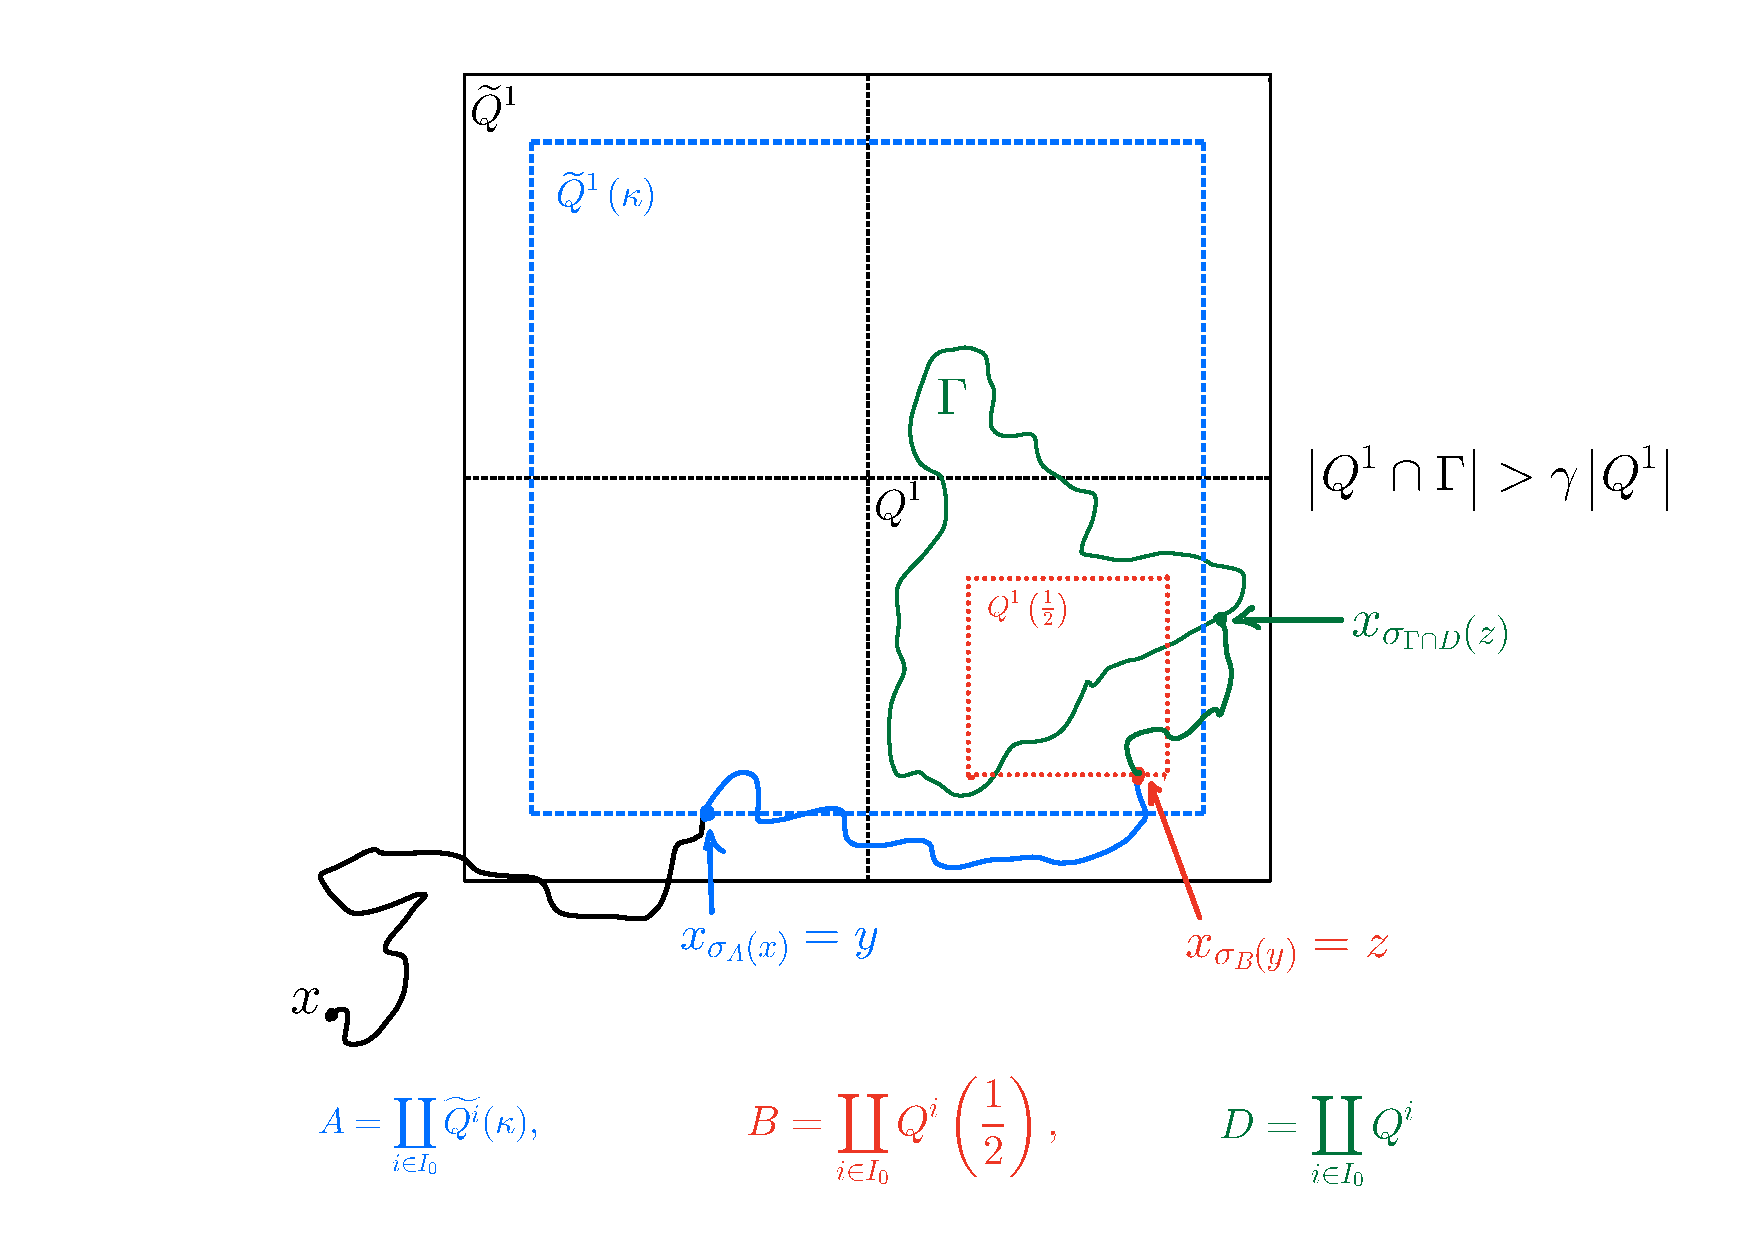
\includegraphics[width=0.9 \textwidth]{hit prob.pdf} 
    \caption{Hitting Prob.} \label{fig:hit} 
    \end{figure}
	
	\section{Harnack Inequality and H\"older estimate}
	In this section, we prove some theorems of Krylov and Safonov \cite{krylov1981certain} concerning (positive) $L$-harmonic functions. Let $\delta\in(0,1)$. Set 
	\begin{align*}
	    \sP(\delta):=\Big\{\{\mP_x\}_{x\in \mR^n}: (\mP_x, X)  \ \textit{is the strong Markov process} \\
        \textit{associate with some } a(\cdot) \in \mS^d_\delta \Big\}.
	\end{align*}
    Let 
    \[
        [u]_{\alpha; D}:=\sup_{x,y\in D} \frac{|u(x)-u(y)|}{|x-y|^\alpha} ~\textit{ and }~ \osc_D u:= \sup_{x\in D} u(x)-\inf_{x\in D} u(x). 
    \]
	
	\begin{theorem}[H\"older estimate]\label{thm:holder}
	  Suppose $u$ is bounded in $Q_1$ and $
	  Lu =0$ in $Q_1$. Then there exist $\alpha$ and $C$ only depending on $d$ and $\delta$ such that
	  \begin{equation}\label{eq:KS-Holder}
	      [u]_{\alpha; Q_{1/2}}\leq C \osc_{Q_1} u.
	  \end{equation} \end{theorem}
	\begin{proof}
  \begin{framed}
      {\bf Claim:} there exists a constant $\rho\in (0,1)$ such that  for any $z\in Q_{1/2}$, $r\leq 1/2$, 
		\begin{equation}\label{eq:osc}
		\osc_{Q_{r/2}(z)} \ u\leq \rho \osc_{Q_{r}(z)} \ u. 
		\end{equation}
  \end{framed}
        Assume the claim is true. Suppose that $x,y\in Q_{1/2}$  and $|x-y|\ll1$, let $k\in \mN$ such that $2^{-k-1}\leq |x-y|< 2^{-k}$. 
        \begin{align*}
            |u(x)-u(y)|\leq& \osc_{Q_{2^{-k}}(x)} u \leq \rho \osc_{Q_{2^{-k+1}}(x)} u \leq \cdots \leq C\rho^k \osc_{Q_1} u\\
            \leq& C \rho^{-\log_2 |x-y|} \osc_{Q_1} u \leq C |x-y|^{-\log_2\rho} \osc_{Q_1} u. 
        \end{align*}
        
        Therefore, the above claim implies \eqref{eq:KS-Holder} with $\alpha=\log_2\rho^{-1}$. 
		
  To prove \eqref{eq:osc}. Without loss of generality, we can assume $\inf_{x\in Q_r(z)}u=0$ and $\sup_{x\in Q_r(z)} u=1$. In this case, $\osc_{Q_{r}(z)} \ u=1$. 
		Let $\Gamma:=\{x\in Q_{r/2}: u(x)\geq 1/2\}$, we may assume $|\Gamma|\geq \frac{1}{2} |Q_{r/2}|$, if not, we replace $u$ by $1-u$. For any $x\in Q_{r/2}$, by  Itô's formula, Theorem \ref{thm:hit} and scaling,  
		\[
            u(x)=\mE_x u(X_{\tau_{Q_r}\wedge \sigma_\Gamma})\geq \frac{1}{2}\mP_x (\sigma_\Gamma<\tau_{Q_{r}})\geq \frac{1}{2} p(2^{-d-1}). 
        \]
        Hence we get 
		$$
		\osc_{Q_{r/2}(z)} u \leq 1-\frac{1}{2}p(2^{-d-1})=:\rho=\rho \osc_{Q_{r}(z)}u. 
		$$
	\end{proof}
	
	
	
	\begin{theorem}[Harnack inequality]\label{thm:harnack}
 Suppose $a\in \mS^d_\delta$ and $L=a_{ij}\p_{ij}$. There exists $C$ depending only on $\delta$ such that if $u$ is nonnegative, bounded in $Q_4$, and $u(X_{t \wedge \tau_{Q_4}})$ is a martingale, then $u(x) \leq C u(y)$ if $x, y \in Q_1$.
    \end{theorem}
    \begin{proof}
        If we look at $u+\delta$ and let $\delta \rightarrow 0$, we may assume $u>0$. By looking at $C u$, we may assume $\inf _{Q_{1/2}} u=1$. By Theorem , we know that $u$ is Hölder continuous in $Q_1$, so there exists
        \[
            y \in Q_{1 / 2} ~\textit{ such that }~ u(y)=1. 
        \]
        We want to show that $u$ is bounded above by a constant in $Q_1$, where the constant depends only on $\delta$.
        
        By the support theorem and scaling, if $x \in Q_{1/2}$, there exists $\delta$ such that 
        \[
            \mathbb{P}_y\left(\sigma_{Q_{1/2}(x)}<\tau_{Q_2}\right) \geq \delta .
        \]
        By scaling, if $z \in Q_{1/2}(x)$, then $\mathbb{P}_z\left(\sigma_{Q_{1/4}(x)}<\tau_{Q_2}\right) \geq \delta$. So by the strong Markov property,
        \[
            \mathbb{P}_z\left(\sigma_{Q_{1/4}(x)}<\tau_{Q_2}\right) \geq \delta^2 .
        \]
        Repeating and using induction,
        \[
            \mathbb{P}_y\left(\sigma_{Q_{2^{-k}}(x)}<\tau_{Q_2}\right) \geq \delta^k .
        \]
        Then
        \[
            \begin{aligned}
                1 & =u(y) \geq \mathbb{E}_y\left[u\left(X_{\sigma_{Q_{2^{-k}}(x)}}\right) ; \sigma_{Q_{2^{-k}}(x)}<\tau_{Q_2}\right] \\
                & \geq \delta^k\left(\inf _{Q_{2^{-k}}(x)} u\right),
            \end{aligned}
        \]
        or 
        \begin{equation}\label{eq:infu-Qk}
            \inf _{Q_{2^{-k}}(x)} u \leq \delta^{-k} , \quad \forall k\geq 1. 
        \end{equation}
        By the proof of Theorem \ref{thm:holder}, there exists $\rho<1$ such that
        \[
             \osc_{Q_{2^{-k-1}}(x)} u\leq \rho \osc_{Q_{2^{-k}}(x)}u .
        \]
        Take $N$ large so that $\rho^{-N} \geq 1/\left(\delta-\delta^2\right)$.  Then
        \[
            \underset{Q_{2^{N-k}}(x)}{\mathrm{Osc}} u \geq \rho^{-N} \underset{Q_{2^{-k}}(x)}{\operatorname{Osc}} u \geq \frac{1}{\delta-\delta^2} \underset{Q_{2^{-k}}(x)}{\operatorname{Osc}} u .
        \]
        Take $K$ large so that $\sqrt{d} 2^{N-K}<1 / 8$. Suppose there exists $x_0 \in Q_1(y)$ such that $u\left(x_0\right) \geq \delta^{-K-1}$. 
        \begin{framed}
            We will construct a sequence $x_1, x_2, \ldots$ by induction such that $u(x_j)\geq \delta^{-K-j-1}$. 
        \end{framed} Suppose we have $x_j \in Q_{2^{N+1-K-j}}\left(x_{j-1}\right)$ with $u\left(x_j\right) \geq \delta^{-K-j-1}$, $j \leq n$. Since $\left|x_j-x_{j-1}\right|<\sqrt{d} 2^{N+1-K-j}, 1 \leq j \leq n$, and $\left|x_0-y\right| \leq 1$, then $\left|x_n-y\right|<2$. Since $u\left(x_n\right) \geq \delta^{-K-n-1}$ and by  \eqref{eq:infu-Qk}, $\inf _{Q_{2^{-K-n}}(x_n)} u \leq \delta^{-K-n}$, 
        $$
            \underset{Q_{2^{-K-n}}(x_n)}{\operatorname{Osc}} u \geq \delta^{-K-n}\left(\delta^{-1}-1\right) .
        $$
        So $\osc_{Q_{2^{N-K-n}}(x_n)} u \geq \delta^{-K-n-2}$, which implies that there exists $x_{n+1} \in$ $Q_{ 2^{N-K-n}}(x_n)$ with $u\left(x_{n+1}\right) \geq \delta^{-K-n-2}$ because $u$ is nonnegative. By induction we obtain a sequence $x_n$ with $x_n \in Q_3(y)$ and $u\left(x_n\right) \rightarrow \infty$. This contradicts the boundedness of $u$ on $Q_4$. Therefore $u$ is bounded on $Q_1$ by $\delta^{-K-1}$.
    \end{proof}
	
